% !TeX root = ../main.tex
\chapter{Introduction and outline}
\label{chap:introduction}

\section{Quantum chromodynamics and its and phase diagram}
\begin{figure}[htp]
    \centering 
    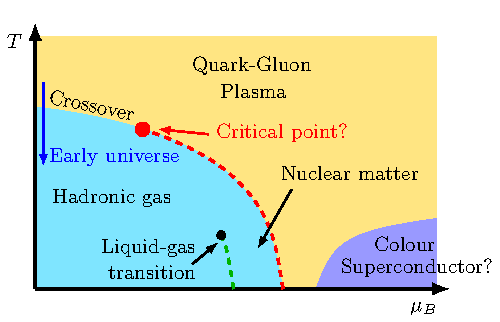
\includegraphics[scale=1.3]{figures/phase_diagram.pdf}
    \caption{Conjectured phase diagram of Quantum Chromodynamics}
    \label{fig:QCD_phase_diagram}
\end{figure}
\textcolor{red}{magari menziona asymptotic freedom?}
Quantum Chromodynamics (QCD) plays fundamental role in our understanding of the Standard Model. It is the theory describing the strong force among quarks and gluons.
The QCD phase diagram, reported in figure \ref{fig:QCD_phase_diagram} as a function of temperature (T) and baryon chemical potential ($\mu_B$), shows
At low temperature and chemical potential QCD exhibits confinement, namely that only colour-neutral states can be observed. The confined phase is characterised by a spontaneously broken chiral symmetry, 
The restoration of chiral symmetry is expected in the transition towards a quark-gluon plasma at high temperatures or chemical potential. Moreoveor, also new states of matter are hypothesed, such as the existence of the colour superconducting state.
The precise determination of the location and nature of the critical point remains an unresolved puzzle, and it's a huge challenge that needs the combination of theory, experiment and simulations.
On the theoretical side, 
The major experiments were performed at the Relativistic Heavy Ion Collider (RHIC) in New York and the Large Hadron
Collider (LHC) at CERN. Another promising experiment, currently under construction, is the Facility for Antiproton
and Ion Research (FAIR) at GSI. On the simulation side, lattice field theory has become the standard approach to study QCD and particle physics.
\section{Lattice Field Theory}
\vspace{20pt}
Computing physical quantities from first principle approaches, is not only hard to do, but results often impossible due to the appearence of divergences in the calculations. To fix this, one often relies on expansion techniques such as perturbation theory (\textcolor{red}{CITATION}), in which one tries to regularise the theory order by order in an expansion on the interaction coupling, yielding finite quantities that depend on the truncation order.  While this method is capable of producing incredibly precise results (\textcolor{red}{g-2, fine structure, ...}), it fails completely in treating non-perturbative phenomena, namely effects that cannot be captured by any order in the expansion or that are typical of strongly interacting systems.
Moreover, such formulation is also not much suitable for numerical computations, since both the path integral and action measure are infinite dimensional objects. \\
Lattice field theory \cite{Montvay1994QuantumLattice,rothe_LGT,gattringer_LQCD,creutz_2023}, which was proposed by Kenneth G. Wilson in 1974 \cite{wilson_lqcd}, is meant at first as a powerful non-perturbative regularisation tool to prevent divergences to occur and render the computation of the correlation functions finite. Moreover, it also provides a framework to study quantum field theory numerically on a computer. In order to accomplish this, one typically defines the theory on a spacetime lattice and makes use of statistical methods such as Monte Carlo algorithms to compute observables. One may wonder how can one reconstruct the results in the continuum theory, keeping the results finite, and matching the results on the discretised theory to physically measured ones. This task, far from beeing simple, will be  discussed in the next chapters, and it will be of one of the motivations for the introduction of coloured noise in the context of the continuum limit of effective theories, a technique which will be shown to be powerful also for other various reasons, which will be the main focus of the analysis carried in the remaining chapters. \\

\section{The emergence of effective theories}
A central role in our investigation will be played by the Wilsonian perspective of the Renormalization Group (RG). Within this paradigm, renormalization ceases to be merely a tool for taming divergences; 
the Wilsonian RG approach provides a way to resolve physics at different scales. The Wilson framework naturally brings to the concept of effective theory, a model which describes phenomena only in terms of relevant degrees of freedom. In the context of QCD, a diverse array of effective theories are introduced, tailored to specific aspects of the strong force dynamics. 
Among others, we mention the Nambu-Jona-Lasinio model \cite{Nambu1961DynamicalI, Nambu1961DynamicalII}, the Gross-Neveu model, the Quark-Meson model. All of these theories are Yukawa-type theories, namely with a fermion-fermion-boson interaction.
\textcolor{red}{magari menziona che Gross Neveu ha applicazioni fuori da QCD}
\newpage 
\section{Outline}
Chapter \ref{chap:background} will be devoted to the introduction of the theoretical background that supports this work. 
We will start with the Kadanoff and Wilson approach to renormalisation in statistical physics and quantum field theory. 
Lattice field theory will then be introduced as a powerfool tool to simulate quantum field theory numerically and the basics of the formulation will be provided. 
We then turn to stochastic quantisation, the relation between noise and quantum fluctuations and how the standard formulation is modified by the presence of coloured noise. 
This will results in a deep connection between coloured stochastic quantisation and the renormalisation group.
The chapter will end with a description of the model on which the above techniques are applied, namely a Yukawa theory. \\~\\
Chapter \ref{chapt:methods} is devoted to detail techniques and methodologies of the project. We will start by explaining how the continuum model is discretised on a space-time lattice and how it can be simulated via a Monte Carlo method and stochastic quantisation. \\
We will then list some possible applications of coloured noise in lattice QFT and describe some of the numerical experiments that will be carried in the last chapter.\\
The chapter will end with a description of the relevant observables that are employed to study a lattice quantum field theory. \\~\\
Chapters \ref{chapt:results_preliminary} and \ref{chapt:results_coloured} are devoted to the numerical investigation. \\
First, some premilinary analysis will be carried. We will show how fermionic masses are measured in the simulation and provide a panoramic over the general phase structure of the theory. The latter will guide the choice of parameter settings for all the simulations. \\
It will then be showed how coloured noise can be used to provide a smooth interpolation between the fully classical and fully quantum picture. \\
The introduction of noise can cause qualitative change in the behaviour of the system. In particular, it will be shown how quantum fluctuations can trigger a chiral phase transition in the model. \\
Finally we will show how coloured noise in combinations with the Kadanoff-Wilson RG can be used to cool a simulation by systematically encoding UV fluctuations in a redefinition of the classical action, without altering the physical content of the theory.